% Pengaturan ukuran teks dan jenis dokumen
\documentclass[11pt]{article}

% Pengaturan ukuran halaman dan margin
\usepackage[a4paper,top=30mm,left=30mm,right=20mm,bottom=20mm]{geometry}

% Pengaturan ukuran spasi
\usepackage[singlespacing]{setspace}

% Judul dokumen
\title{Proposal Tugas Akhir ITS}
\author{Maulana, Alfi}

% Pengaturan format bahasa
\usepackage[indonesian]{babel}

% Pengaturan detail pada file PDF
\usepackage[pdfauthor={\@author},bookmarksnumbered,pdfborder={0 0 0}]{hyperref}

% Pengaturan jenis karakter
\usepackage[utf8]{inputenc}

% Pengaturan ukuran indentasi
\setlength{\parindent}{2em}

% Package lainnya
\usepackage{etoolbox} % Mengubah fungsi default
\usepackage{enumitem} % Pembuatan list
\usepackage{lipsum} % Pembuatan template kalimat
\usepackage{graphicx} % Input gambar
\usepackage{longtable} % Pembuatan tabel
\usepackage[table,xcdraw]{xcolor} % Pewarnaan tabel
\usepackage[numbers]{natbib} % Kutipan artikel
\usepackage{changepage} % Pembuatan teks kolom
\usepackage{multicol} % Pembuatan kolom ganda
\usepackage{multirow} % Pembuatan baris ganda

% Pengaturan format judul bab
\usepackage{titlesec}
\renewcommand{\thesection}{\arabic{section}}
\titleformat*{\section}{\normalsize\bfseries}
\titleformat*{\subsection}{\normalsize\bfseries}
\titlespacing{\section}{0ex}{3ex}{1.5ex}
\titlespacing{\subsection}{0ex}{3ex}{1.5ex}

% Isi keseluruhan dokumen
\begin{document}

  % Menonaktifkan penomoran halaman
  \pagenumbering{gobble}

  % Lembar pengesahan
  \begin{flushleft}
  % Ubah kalimat berikut sesuai dengan nama departemen dan fakultas
  \textbf{Departemen Teknik Komputer - FTEIC}\\
  % Ubah kalimat berikut sesuai dengan nama universitas
  \textbf{Institut Teknologi Sepuluh Nopember}\\
\end{flushleft}

\begin{center}
  % Ubah detail mata kuliah berikut sesuai dengan yang ditentukan oleh departemen
  \underline{\textbf{EC184701 - PRA TUGAS AKHIR - 2 SKS}}
\end{center}

\begin{adjustwidth}{-0.2cm}{}
  \begin{tabular}{lcp{0.7\linewidth}}

    % Ubah kalimat-kalimat berikut sesuai dengan nama dan NRP mahasiswa
    Nama Mahasiswa &:& Muhammad Alfi Maulana Fikri \\
    Nomor Pokok &:&	0721 17 4000 0009 \\

    % Ubah kalimat berikut sesuai dengan semester pengajuan proposal
    Semester &:& Ganjil 2020/2021 \\

    % Ubah kalimat-kalimat berikut sesuai dengan nama-nama dosen pembimbing
    Dosen Pembimbing &:& 1. Prof. Dr. Ir. Mauridhi Hery Purnomo, M.Eng. \\
    & & 2. Dr. I Ketut Eddy Purnama, ST., MT. \\

    % Ubah kalimat berikut sesuai dengan judul tugas akhir
    Judul Tugas Akhir &:& \textbf{Desain dan Implementasi Simulasi Untuk \emph{Socially Assistive Robots} Menggunakan \emph{ROS 2}} \\

    Uraian Tugas Akhir &:& \\
  \end{tabular}
\end{adjustwidth}

% Ubah paragraf berikut sesuai dengan uraian dari tugas akhir
\lipsum[1]
\vspace{1ex}

\begin{flushright}
  % Ubah kalimat berikut sesuai dengan tempat, bulan, dan tahun penulisan
  Surabaya, Desember 2020
\end{flushright}
\vspace{1ex}

\begin{center}

  \begin{multicols}{2}

    Dosen Pembimbing 1
    \vspace{12ex}

    % Ubah kalimat-kalimat berikut sesuai dengan nama dan NIP dosen pembimbing pertama
    \underline{Prof. Dr. Ir. Mauridhi Hery P., M.Eng.} \\
    NIP. 19580916 198601 1 001

    \columnbreak

    Dosen Pembimbing 2
    \vspace{12ex}

    % Ubah kalimat-kalimat berikut sesuai dengan nama dan NIP dosen pembimbing kedua
    \underline{Dr. I Ketut Eddy P., S.T., M.T.} \\
    NIP. 19690730 199512 1 001

  \end{multicols}
  \vspace{6ex}

  Mengetahui, \\
  % Ubah kalimat berikut sesuai dengan jabatan kepala departemen
  Kepala Departemen Teknik Komputer FTEIC - ITS
  \vspace{12ex}

  % Ubah kalimat-kalimat berikut sesuai dengan nama dan NIP kepala departemen
  \underline{Dr. Supeno Mardi Susiki Nugroho, S.T., M.T.} \\
  NIP. 19700313 199512 1 001

\end{center}

  \newpage

  % Konten pendahuluan
  \section{PENDAHULUAN}

\subsection{Latar Belakang}

Selama beberapa tahun belakang, robot telah mengalami perkembangan yang cukup signifikan dari robot besar untuk industri hingga robot kecil yang membantu pekerjaan ringan rumah tangga.
Salah satu jenis robot yang belakangan ini mulai banyak dikembangkan tersebut adalah \emph{socially assistive robots} (\emph{SARs}).
\emph{SARs} sendiri merupakan jenis robot yang membantu manusia melalui interaksi sosial seperti sebagai robot untuk pendamping maupun pelayan.

Dalam pengembangannya, seringkali pengujian suatu robot, termasuk \emph{SARs}, mengalami kendala karena pengujian secara langsung beresiko merusak \emph{hardware} yang mahal.
Selain itu robot yang dikembangkan juga akan lebih sulit untuk diubah desainnya karena pengubahan desain pada robot langsung akan memakan lebih banyak waktu dan biaya.

Salah satu solusi untuk mengatasi masalah tersebut adalah dengan menggunakan simulasi robot.
Simulasi robot sendiri merupakan simulasi yang digunakan untuk mensimulasikan \emph{physical robot} tanpa bergantung terhadap \emph{hardware} dari robot tersebut, sehingga bisa menghemat biaya dan waktu.
Untuk saat ini, sudah banyak aplikasi yang bisa digunakan untuk mensimulasikan robot tersebut seperti \emph{Gazebo}, \emph{V-Rep}, \emph{Webots}, \emph{Isaac Sim}, dan lain sebagainya.

Namun kendala dari simulasi yang umumnya digunakan saat ini adalah ketika mengembangkan program robot yang ada di simulasi, untuk membawanya ke robot aslinya maka diperlukan pemrograman ulang untuk robot tersebut.
Walaupun begitu, beberapa simulasi seperti \emph{Webots} dan \emph{Isaac Sim} mengatasi masalah tersebut dengan membuat \emph{compiler} yang mampu mengubah program yang ada di simulasi ke program yang ada di robot.
Namun kendala dari metode \emph{compiler} tersebut adalah keterbatasan robot yang bisa di-\emph{compile}, hanya robot komersial seperti \emph{Nao}, \emph{Turtlebot}, dan lain sebagainya yang bisa diubah dari simulasi ke robot aslinya.

Untuk mengatasi masalah tersebut, terutama untuk pengembangan robot kustom yang dibuat sendiri, maka di penelitian ini saya merumuskan desain dan implementasi simulasi terutama untuk \emph{socially assistive robots} sehingga program yang ada di robot tersebut dapat dengan mudah digunakan di simulasi maupun robot aslinya.

\subsection{Rumusan Masalah}

Dari pemaparan yang telah dijelaskan di bagian latar belakang, dapat disimpulkan bahwa pengujian \emph{SARs} secara langsung pada manusia memiliki resiko yang besar terhadap keselamatan manusia serta besarnya biaya yang diperlukan untuk pengembangan dan pengujian robot.

\subsection{Penelitian Terkait}

Takaya et al. \citep{Takaya2016} mengembangkan lingkungan simulasi untuk pengujian terhadap \emph{mobile robot} menggunakan \emph{ROS} dan \emph{Gazebo}.
Sebelumnya penelitian yang sama juga dilakukan oleh Qian et al. \citep{Qian2014} untuk robot berjenis \emph{manipulator} dan Zhang et al. \citep{Zhang2015} untuk robot berjenis \emph{quadrotor UAV}.

Erickson et al. \citep{Erickson2020} mengembangkan \emph{framework} simulasi berbasis \emph{OpenAI Gym} \citep{Brockman2016} untuk \emph{assistive robotics}.
\emph{Framework} simulasi tersebut kemudian digunakan oleh Clegg et al. \citep{Clegg2020} untuk mengembangkan metode \emph{learning} pada kolaborasi antara robot dengan manusia dalam membantu pemakaian baju pada manusia.
Selain itu penelitian yang dilakukan Zamora et al. \citep{Zamora2016} menunjukkan simulasi pada \emph{OpenAI Gym} bisa digunakan bersamaan dengan \emph{ROS} dan \emph{Gazebo}.

\subsection{Tujuan Penelitian}

Tujuan dari penelitian ini adalah untuk mengembangkan lingkungan simulasi yang bisa digunakan untuk melakukan pengujian terhadap \emph{SARs} secara virtual, sebagai alternatif dari pengujian terhadap \emph{SARs} secara langsung.

  % Konten tinjauan pustaka
  \section{TINJAUAN PUSTAKA}

\subsection{\emph{Socially Assistive Robots}}

\begin{figure} [ht] \centering
  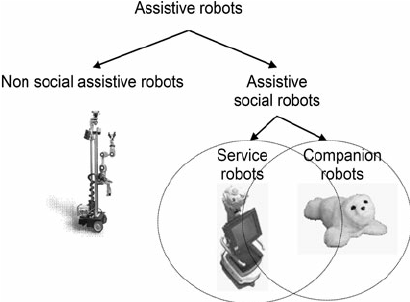
\includegraphics[scale=0.50]{gambar/robots-category.png}
  \caption{Pengategorian \emph{assistive robots} menurut Heerink et al. \citep{Heerink2010}}
  \label{fig:RobotsCategory}
\end{figure}

\emph{Socially assistive robots} (SARs) merupakan adaptasi dari \emph{assistive technology} yang meliputi keseluruhan sistem robotika yang mampu memberikan bantuan kepada pengguna dalam bentuk interaksi sosial \citep{Seifer2005}. Heerink et al. \citep{Heerink2010} mengategorikan riset terhadap SARs menjadi dua kategori berbeda seperti pada Gambar \ref{fig:RobotsCategory}.
Kategori pertama mencakup \emph{service robots} yang menawarkan bantuan fisik dan kognitif dan melakukan tugas sebagai pelayan, sedangkan kategori kedua mencakup \emph{companion robot} yang merupakan robot berjenis pendamping sebagai sahabat dan media untuk terapi.
Lebih lanjut Rich et al. \citep{Rich2009} menjelaskan SARs mampu memberikan bantuan kepada pengguna dalam berbagai tingkatan seperti:
(a) mendukung kemampuan fungsional dan kognitif pengguna;
(b) menawarkan pengguna kesempatan untuk meningkatkan partisipasi sosial dan kesehatan psikologis;
(c) menyediakan pemantauan jarak jauh dan berkelanjutan atas status kesehatan pengguna;
dan (d) membina pengguna untuk memfasilitasi promosi perilaku sehat dan pencapaian tujuan yang berhubungan dengan kesehatan.

\subsection{Robot Operating System 2 (ROS 2)}

Robot Operating System (ROS) \citep{Quigley2009} merupakan kumpulan dari libraries, drivers, dan tools yang mempermudah pengembangan sistem pada robot.
ROS memiliki command tool seperti Linux, sistem komunikasi antar proses, dan berbagai macam packages yang berhubungan dengan pengembangan sistem pada robot.
Proses yang dieksekusi pada ROS disebut sebagai Node, komunikasi antar proses yang dimiliki menggunakan model \emph{publish/subscribe}, dan data komunikasi yang dikirimkan disebut sebagai Topic.
Suatu proses Publisher mampu mengirimkan satu maupun lebih Topic, kemudian proses-proses lain yang melakukan subscribe pada suatu Topic bisa memperoleh isi dari Topic tersebut.
Selain itu ada juga Sevice yang memiliki fungsi seperti Topic, hanya saja dilakukan secara dua arah.
Service ini bekerja menggunakan model \emph{client/server} dimana Service Client akan mengirimkan data permintaan dalam bentuk Request dan kemudian Service Server akan mengirimkan data balasan dalam bentuk Response.

Generasi kedua dari Robot Operating System, ROS 2, merupakan kelanjutan dari ROS yang mengusung reliabilitas dan performa untuk penggunaan \emph{real-time} sembari masih mendukung keunggulan yang dimiliki oleh ROS sebelumnya \citep{Maruyama2016}.
Untuk memenuhi kebutuhan reliabilitas dan performa untuk penggunaan real-time tersebut, ROS 2 menggunakan \emph{Data Distribution Service} (DDS) \citep{Castellote2003} \citep{Schlesselman2004}, standar industri untuk sistem komunikasi real-time dan \emph{end-to-end middleware}, yang menggantikan sistem komunikasi antar proses yang dimiliki ROS sebelumnya.

\subsection{Gazebo}

Gazebo \citep{Koenig2004} merupakan bagian dari Player Project \citep{Gerkey2003} yang memungkinkan sebuah simulasi robot dan aplikasi sensor bekerja di lingkungan simulasi indoor maupun outdoor tiga dimensi.
Gazebo memiliki arsitektur \emph{client/server} dan model \emph{publish/subscribe} untuk sistem komunikasi antar prosesnya.
Setiap objek simulasi di Gazebo dapat diasosiasikan dalam satu maupun lebih kontroler yang akan memproses perintah untuk mengatur dan menentukan keadaan dari suatu objek.
Data yang dihasilkan oleh suatu kontroler akan dikirim ke \emph{shared memory} menggunakan Gazebo interfaces (ifaces).
Nantinya ifaces dari proses-proses lain dapat membaca data tersebut pada shared memory, sehingga memungkinkan komunikasi antar proses antara program yang mengontrol robot dan Gazebo, terlepas dari bahasa pemrograman yang digunakan.


  % Konten metodologi
  \section{METODOLOGI}

\subsection{Desain Robot yang Digunakan}

\begin{figure} [ht] \centering
	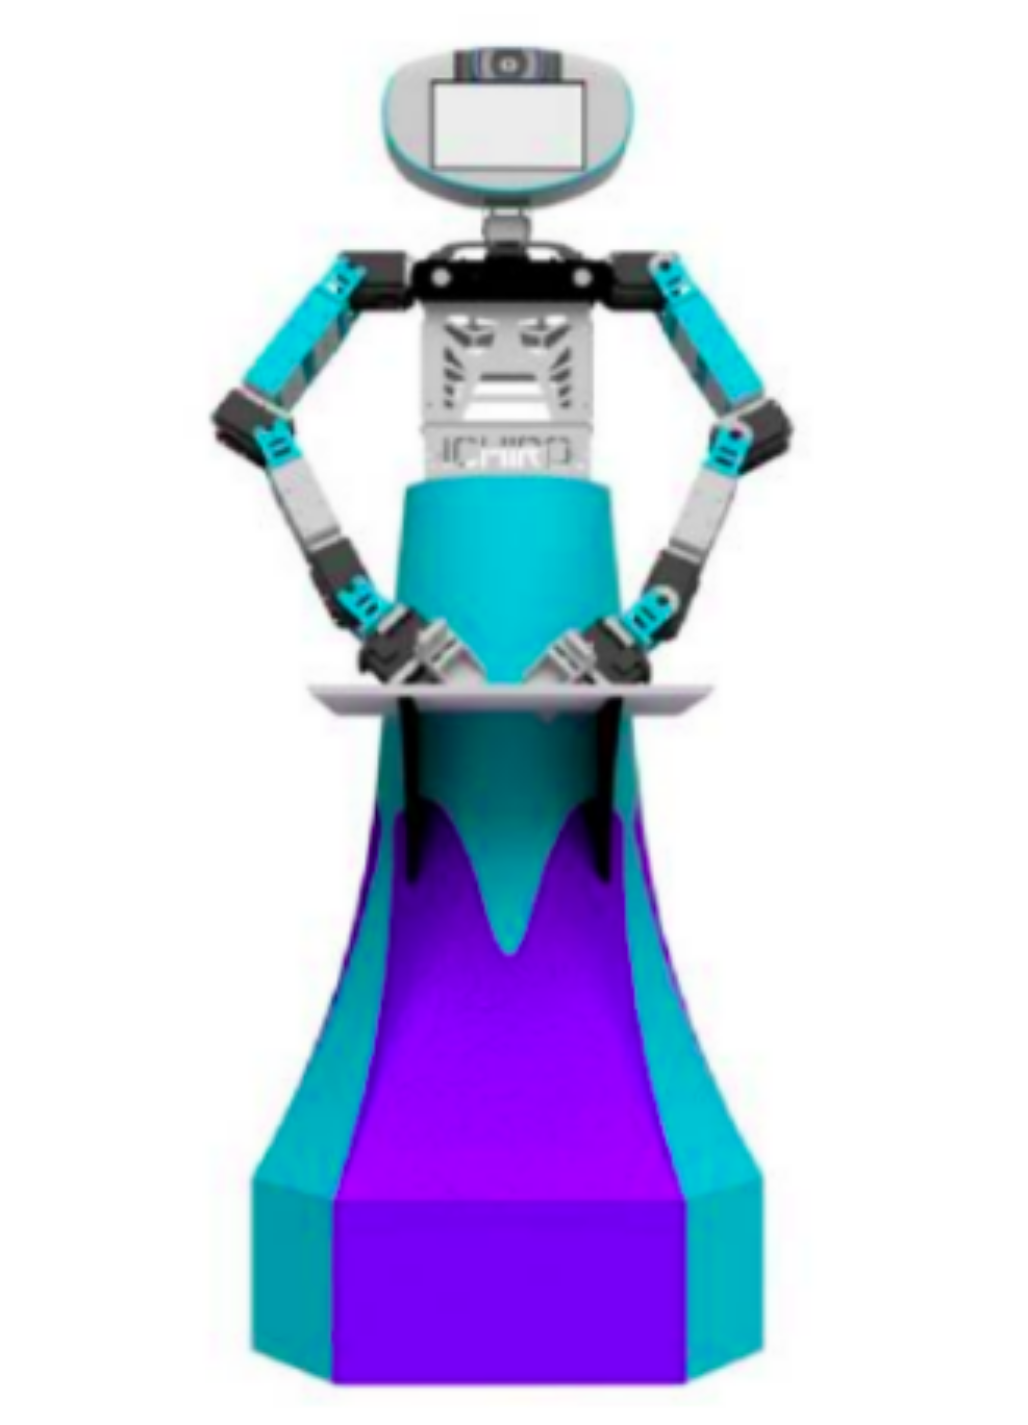
\includegraphics[scale=0.45]{gambar/robot-design.png}
	\caption{Desain Robot yang Digunakan}
	\label{fig:RobotDesign}
\end{figure}

Robot yang akan digunakan pada pada penelitian ini memiliki desain \emph{mobile humanoid robot} \citep{Mohamed2012}, yang merupakan gabungan antara robot mobile dan robot humanoid.
Seperti yang terlihat pada gambar \ref{fig:RobotDesign}, bagian bawah robot menyerupai robot mobile dengan \emph{differential wheels} yang memungkinkan pergerakan ke segala arah secara dua dimensi, sedangkan bagian atas robot menyerupai robot humanoid yang terdiri atas badan, kepala, dan lengan.
Dengan desain mobile humanoid robot ini, diharapkan pengguna bisa merasakan interaksi sosial yang lebih baik dengan robot karena memiliki bentuk mendekati manusia \citep{Rossi2018} sambil mempermudah navigasi dari robot ke berbagai tempat.

Robot ini dilengkapi dengan beberapa sensor seperti IMU (\emph{inertial measurement unit}) untuk mengetahui orientasi dari robot dan sensor kamera di kepala untuk mendeteksi objek menggunakan visi komputer.
Selain itu robot ini juga dilengkapi dengan dua lengan seperti robot manipulator yang bisa diatur pada berbagai posisi dan orientasi \citep{Iqbal2012}.
Dengan adanya sensor dan lengan ini diharapkan robot mampu melakukan tindakan assistive secara sosial sesuai dengan data yang didapatkan dari sensor yang ada.

\subsection{Pengembangan Controller Robot}

\begin{figure} [ht] \centering
	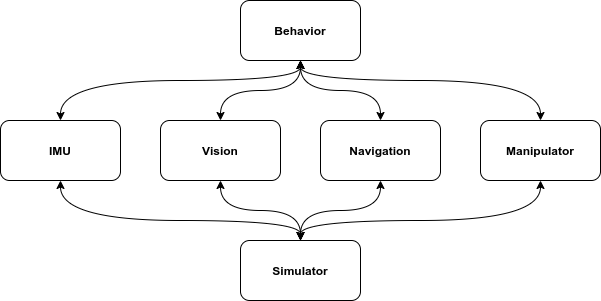
\includegraphics[scale=0.45]{gambar/robot-controller.png}
	\caption{Diagram sistem controller robot}
	\label{fig:RobotController}
\end{figure}

Controller robot yang digunakan untuk simulasi akan dikembangkan menggunakan ROS 2.
Controller tersebut akan dipisah menjadi beberapa node seperti yang terlihat pada gambar \ref{fig:RobotController}.
Setiap node yang ada akan terhubung satu sama lain menggunakan sistem komunikasi antar proses ROS 2 yang berupa topics dan services.

Bagian utama dari controller robot tersebut adalah node Behavior yang berisi program yang mengatur segala tindakan robot berdasarkan data yang didapat dari sensor yang ada di simulasi.
Kemudian node Behavior tersebut akan terhubung dengan empat node lain yang merepresentasikan sensor dan aktuator yang ada pada robot.
Keempat node tersebut adalah node IMU yang akan memproses data dari sensor IMU yang ada di robot, node Vision yang akan memproses program visi komputer menggunakan gambar yang didapat dari kamera robot, node Navigation yang mengatur pergerakan robot, dan node Manipulator yang mengatur posisi dan orientasi dari lengan robot.
Terakhir, keempat node sensor dan aktuator tersebut akan terhubung dengan node Simulator, yang dalam hal ini adalah simulator Gazebo.

\subsection{Pembuatan Lingkungan Simulasi}

Lingkungan simulasi dibuat menggunakan \emph{Gazebo}.

\subsection{Pengujian Sistem Robot terhadap Lingkungan Simulasi}

Pengujian sistem robot akan dilakukan untuk setiap fungsionalitas yang dimiliki robot.


  % Konten lainnya
  \section{HASIL YANG DIHARAPKAN}

\subsection{Hasil yang Diharapkan dari Penelitian}

Dari penelitian yang akan dilakukan, diharapkan dapat menghasilkan sebuah lingkungan simulasi yang mampu digunakan untuk melakukan pengujian pada \emph{Socially Assistive Robots} (SARs) secara virtual menggunakan simulasi robot, sebagai alternatif dari pengujian yang secara langsung menguji pengguna dengan robot fisik.
Dari penelitian ini juga diharapkan pengembangan pada SARs bisa dilakukan dengan lebih mudah karena dapat meminimalisir resiko, mengurangi biaya, serta menghemat waktu dari pengujian yang dilakukan pada SARs.

\subsection{Hasil Pendahuluan}

Desain 3D berbasis CAD dari robot yang akan kami gunakan sudah ada seperti yang terlihat pada Gambar \ref{fig:RobotDesign}, yang perlu dilakukan adalah mengubah desain tersebut mengikuti format SDF yang ada pada simulator Gazebo.
Untuk simulator Gazebo tersebut sendiri sudah kami coba menggunakan contoh lingkungan simulasi yang sudah ada.
Dari lingkungan simulasi tersebut nantinya akan dikembangkan lebih lanjut menjadi lingkungan simulasi yang menyesuaikan dengan pengujian yang akan dilakukan.

Terkait dengan kontroler robot untuk simulasi, sebelumnya kontroler semacam itu sudah pernah kami buat menggunakan ROS 2 untuk simulator Webots dengan desain robot yang lain.
Struktur yang ada pada kontroler tersebut juga sama dimana terpisah menjadi sebuah node behavior dan beberapa node lain yang memproses sensor maupun aktuator yang ada di lingkungan simulasi.
Yang perlu dilakukan adalah menyesuaikan kontroler dengan struktur tersebut agar bisa digunakan dengan simulator Gazebo, serta mengatur sensor dan aktuator yang digunakan di simulasi menyesuaikan sensor dan aktuator yang digunakan pada robot yang diujikan di penelitian ini.

\section{RENCANA KERJA}

\newcommand{\w}{}
\newcommand{\G}{\cellcolor{gray}}
\begin{table}[h!]
  \begin{tabular}{|p{42mm}|c|c|c|c|c|c|c|c|c|c|c|c|c|c|c|c|}

    \hline
    \multirow{2}{*}{Kegiatan} & \multicolumn{16}{|c|}{Minggu} \\
    \cline{2-17} &
    1 & 2 & 3 & 4 & 5 & 6 & 7 & 8 & 9 & 10 & 11 & 12 & 13 & 14 & 15 & 16 \\
    \hline

    Pembuatan lingkungan simulasi &
    \G & \G & \G & \G & \G & \G & \w & \w & \w & \w & \w & \w & \w & \w & \w & \w \\
    \hline

    Pengembangan kontroler robot &
    \w & \w & \G & \G & \G & \G & \G & \G & \G & \G & \G & \G & \G & \G & \w & \w \\
    \hline

    Pengujian robot pada lingkungan simulasi &
    \w & \w & \w & \w & \w & \w & \w & \w & \G & \G & \G & \G & \w & \w & \w & \w \\
    \hline

    Pemindahan kontroler ke robot fisik &
    \w & \w & \w & \w & \w & \w & \w & \w & \w & \w & \w & \w & \G & \G & \w & \w \\
    \hline

    Evaluasi hasil pengujian &
    \w & \w & \w & \w & \w & \w & \w & \w & \w & \w & \w & \w & \w & \w & \G & \G \\
    \hline

  \end{tabular}
\end{table}


  % Daftar pustaka
  \section{DAFTAR PUSTAKA}
  \renewcommand\refname{}
  \vspace{-2ex}
  % \nocite{*}
  \bibliographystyle{unsrtnat}
  \bibliography{pustaka/pustaka.bib}

\end{document}
